\documentclass[xcolor=pdftex,dvipsnames,table,mathserif,aspectratio=169]{beamer}
\usetheme{default}
%\usetheme{Darmstadt}
%\usepackage{times}
%\usefonttheme{structurebold}

\usepackage[english]{babel}
%\usepackage[table]{xcolor}
\usepackage{pgf,pgfarrows,pgfnodes,pgfautomata,pgfheaps}
\usepackage{amsmath,amssymb,setspace,centernot}
\usepackage[latin1]{inputenc}
\usepackage[T1]{fontenc}
\usepackage{relsize}
\usepackage{pdfpages}
\usepackage[absolute,overlay]{textpos} 
\usepackage{listings}




\newenvironment{reference}[2]{% 
  \begin{textblock*}{\textwidth}(#1,#2) 
      \footnotesize\it\bgroup\color{red!50!black}}{\egroup\end{textblock*}} 

\DeclareMathSizes{10}{10}{6}{6} 

\begin{document}
\title{Part 4: Binary Choice}
\author{Chris Conlon}
\institute{Microeconometrics}
\date{\today}

\frame{\titlepage}

\section{Intro}

\begin{frame}
\frametitle{Binary Choice: Overview}
Many problems we are interested in look at discrete rather than continuous outcomes:
\begin{itemize}
\item Entering a Market/Opening a Store
\item Working or a not
\item Being married or not
\item Exporting to another country or not
\item Going to college or not
\item Smoking or not
\item etc.
\end{itemize}
\end{frame}

\begin{frame}
\frametitle{Simplest Example: Flipping a Coin}
Suppose we flip a coin which is yields heads ($Y=1$) and tails ($Y=0$). We want to estimate the probability $p$ of heads:
\begin{eqnarray*}
Y_i =
\begin{cases}
1 \mbox{ with probability } p \\
0 \mbox{ with probability } 1-p
\end{cases}
\end{eqnarray*}
We see some data $Y_1,\ldots,Y_N$ which are (i.i.d.)\\
\vspace{0.2cm}
We know that $Y_i \sim Bernoulli(p)$.
\end{frame}


\begin{frame}{Simplest Example: Flipping a Coin}
We can write the likelihood of $N$ Bernoulli trials as 
$$Pr(Y_1 = y_1, Y_2=y_2,\ldots,Y _N=y_N )  =  f(y_1,y_2,\ldots,y_N | p ) $$
\begin{eqnarray*}
&=& \prod_{i=1}^N p^{y_i} (1-p)^{1-y_i}\\
&=& p^{\sum_{i=1}^N y_i} (1-p)^{N-\sum{i=1}^N y_i}
\end{eqnarray*}
And then take logs to get the \alert{log likelihood}:
\begin{eqnarray*}
\ln  f(y_1,y_2,\ldots,y_N | p )  &=& \left( \sum_{i=1}^N y_i \right)  \ln p  + \left(N-\sum_{i=1}^N y_i \right)  (1-p)
\end{eqnarray*}
\end{frame}

\begin{frame}{Simplest Example: Flipping a Coin}
Differentiate the log-likelihood to find the maximum:
\begin{eqnarray*}
\ln  f(y_1,y_2,\ldots,y_N | p )  &=& \left( \sum_{i=1}^N y_i \right)  \ln p  + \left(N-\sum_{i=1}^N y_i \right)  (1-p)\\
\rightarrow 0&=& \frac{1}{\hat{p}}  \left( \sum_{i=1}^N y_i \right) + \frac{-1}{1-\hat{p}}   \left(N-\sum_{i=1}^N y_i \right) \\
 \frac{\hat{p}}{1-\hat{p}} &=& \frac{\sum_{i=1}^N y_i }{N- \sum_{i=1}^N y_i } = \frac{\overline{Y}}{1-\overline{Y}} \\
\hat{p}^{MLE} &=& \overline{Y}
\end{eqnarray*}
That was a lot of work to get the obvious answer: \alert{fraction of heads}.
\end{frame}

\begin{frame}{More Complicated Example: Adding Covariates}
We probably are interested in more complicated cases where $p$ is not the same for all observations but rather $p(X)$ depends on some covariates. Here is an example from the Boston HMDA Dataset:
\begin{itemize}
\item 2380 observations from 1990 in the greater Boston area.
\item Data on: individual Characteristics, Property Characteristics, Loan Denial/Acceptance (1/0).
\item Mortgage Application process circa 1990-1991:
\begin{itemize}
\item Go to bank
\item Fill out an application (personal+financial info)
\item Meet with loan officer
\item Loan officer makes decision
\begin{itemize}
\item Legally in race blind way (discrimination is illegal but rampant)
\item Wants to maximize profits (ie: loan to people who don't end up defeaulting!)
\end{itemize}
\end{itemize}
\end{itemize}
\end{frame}


\begin{frame}{Loan Officer's Decision}
Financial Variables:
\begin{itemize}
\item $P/I$ ratio
\item housing expense to income ratio
\item loan-to-value ratio
\item personal credit history (FICO score, etc.)
\item Probably some nonlinearity:
\begin{itemize}
\item Very high $LTV > 80\%$ or $>95\%$ is a bad sign (strategic defaults?)
\item Credit Score Thresholds
\end{itemize}
\end{itemize}
\end{frame}


\begin{frame}{Loan Officer's Decision}
Goal $Pr(Deny=1 | black, X)$\\

\begin{itemize}
\item Lots of potential \alert{omitted variables} which are correlated with race
\begin{itemize}
\item Wealth, type of employment
\item family status
\item credit history
\item zip code of property
\end{itemize}
\item Lots or \alert{redlining} cases hinge on whether or not black applicants were treated in a discriminatory way.
\end{itemize}
\end{frame}

\begin{frame}
\begin{center}
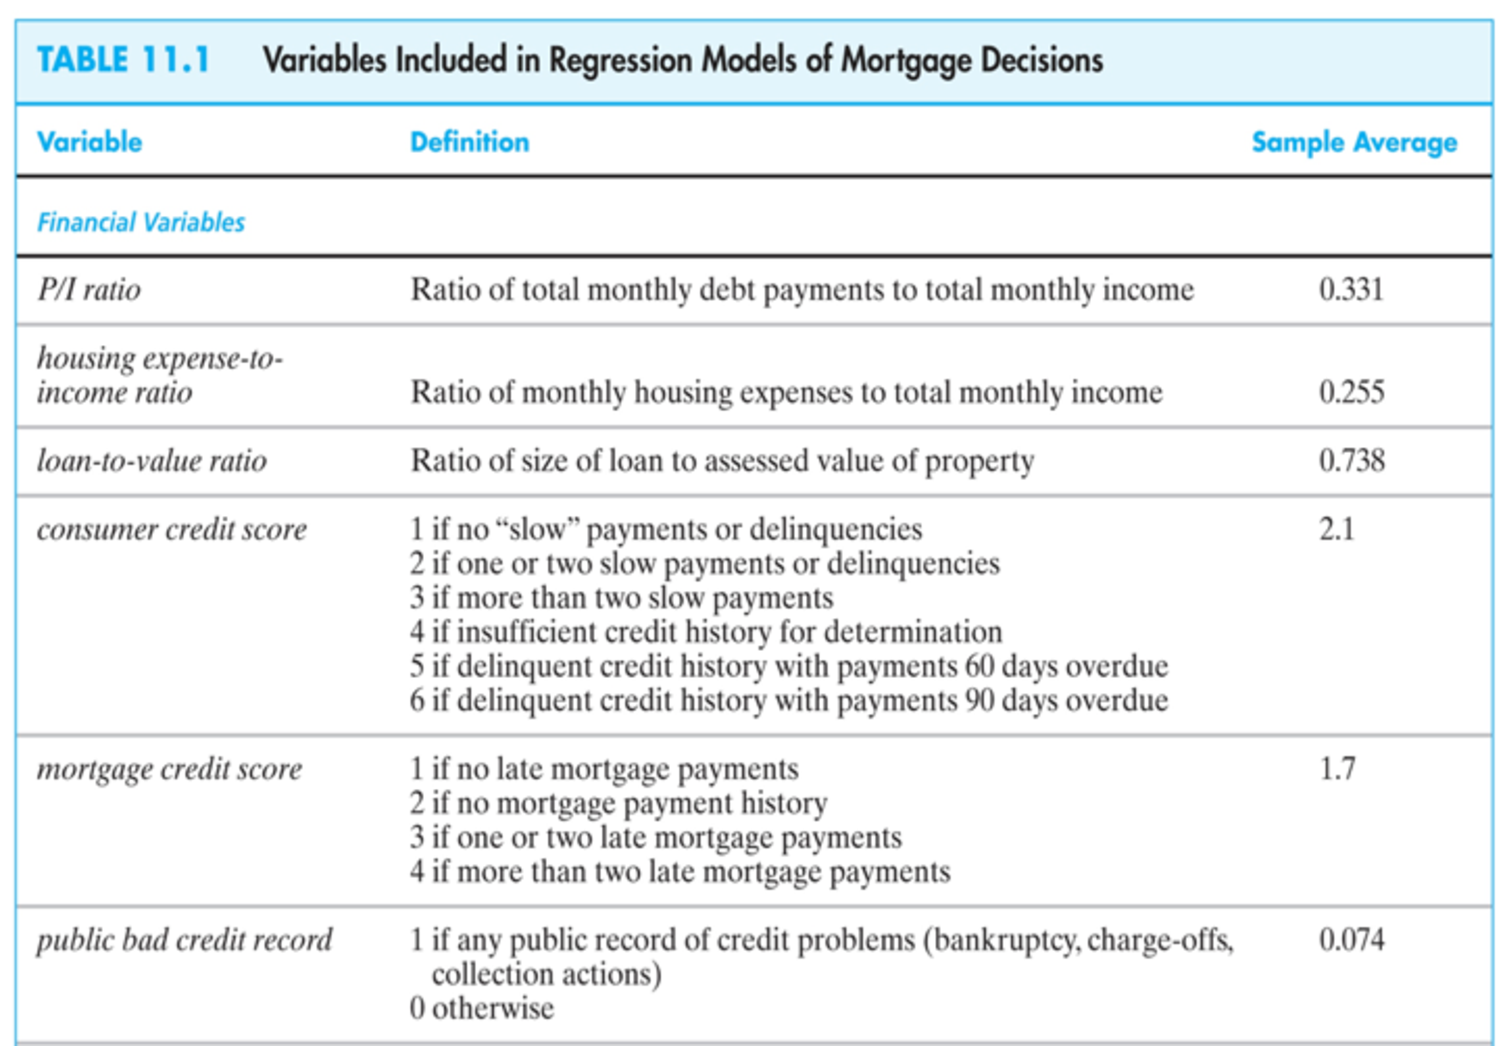
\includegraphics[width=3.25in]{resources/hmda1.pdf}\\
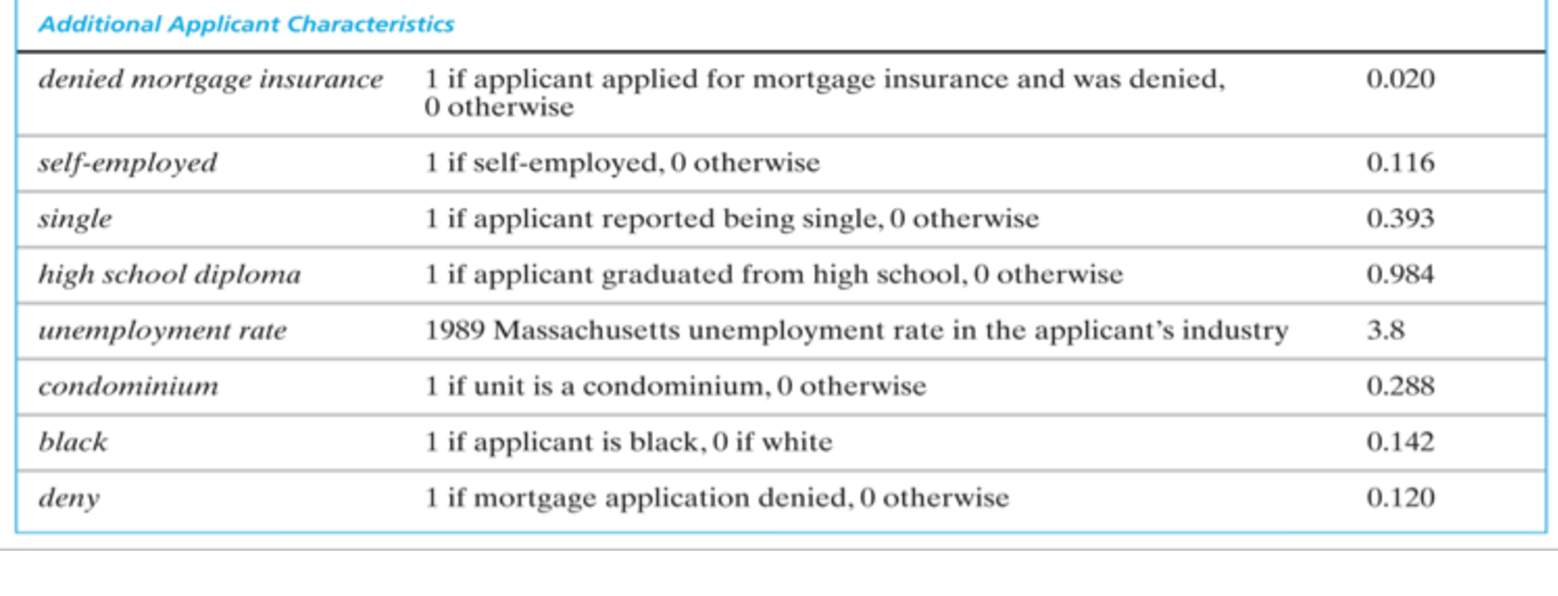
\includegraphics[width=3.25in]{resources/hmda2.pdf}
\end{center}
\end{frame}

\begin{frame}
\begin{center}
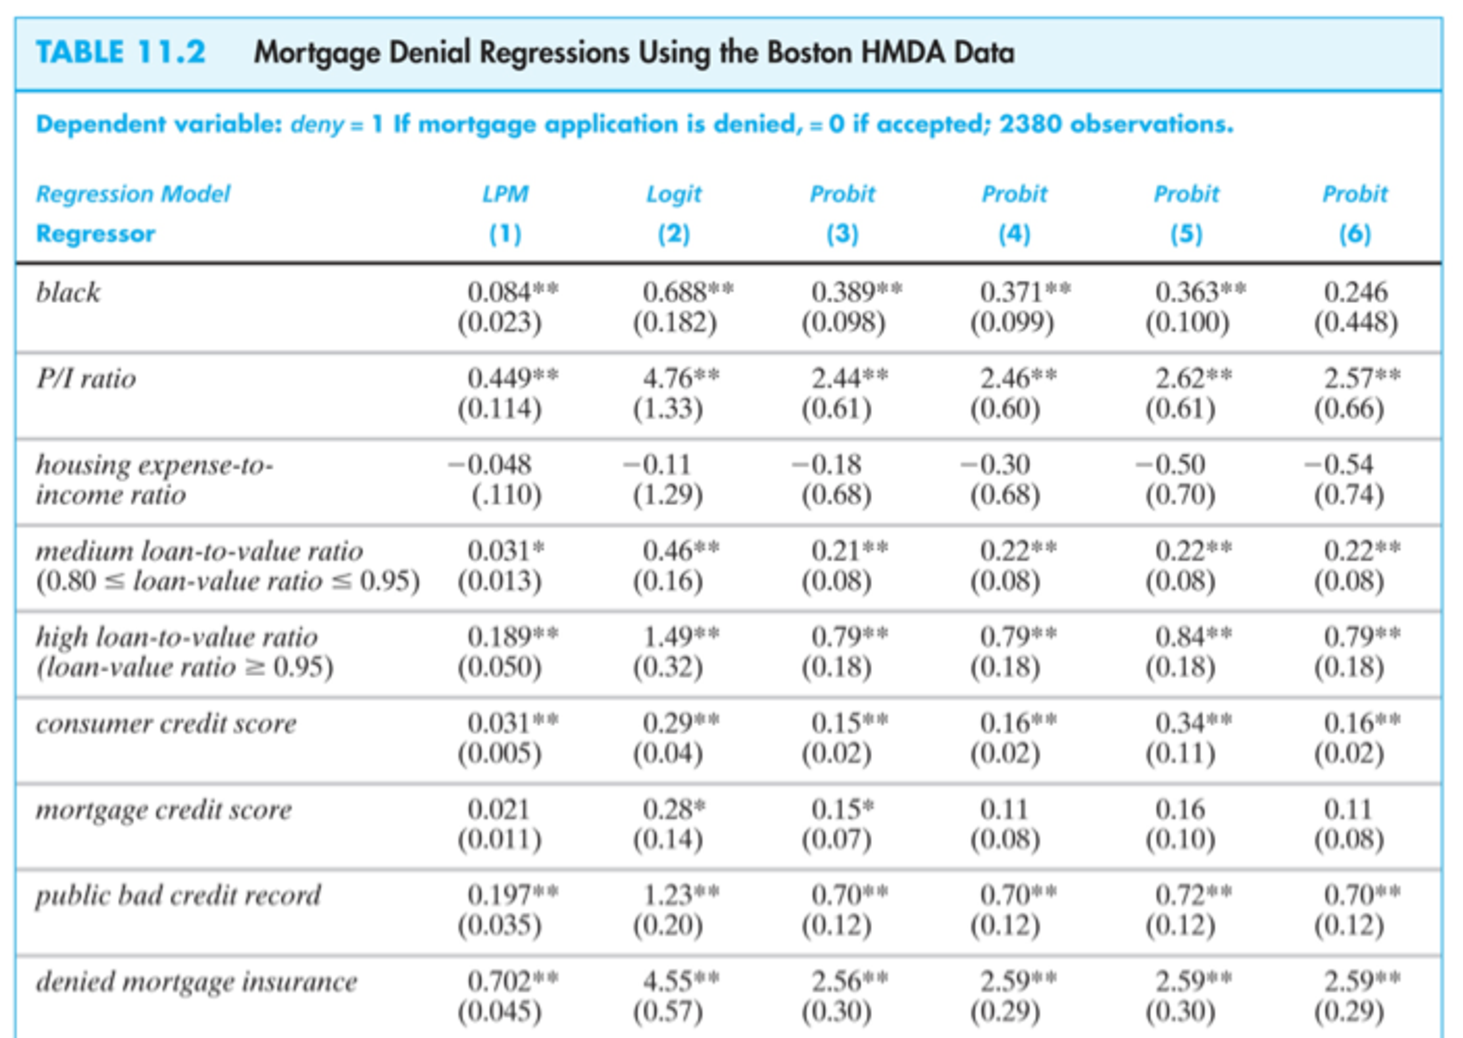
\includegraphics[width=2.5in]{resources/hmda3.pdf}\\
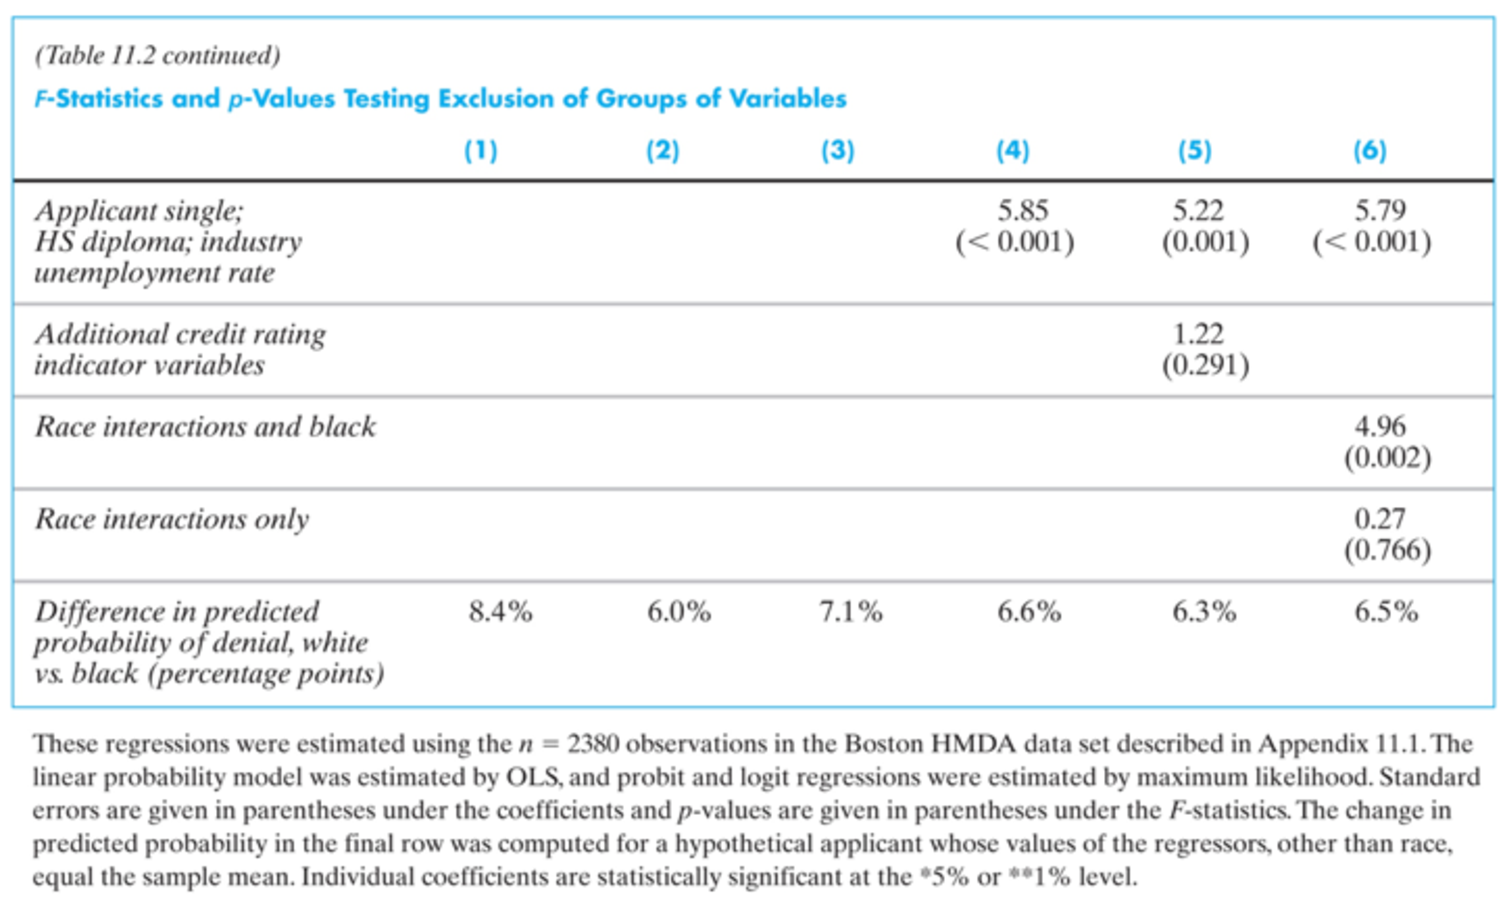
\includegraphics[width=2.5in]{resources/hmda3a.pdf}\\
\end{center}
\end{frame}





\begin{frame}
\begin{center}
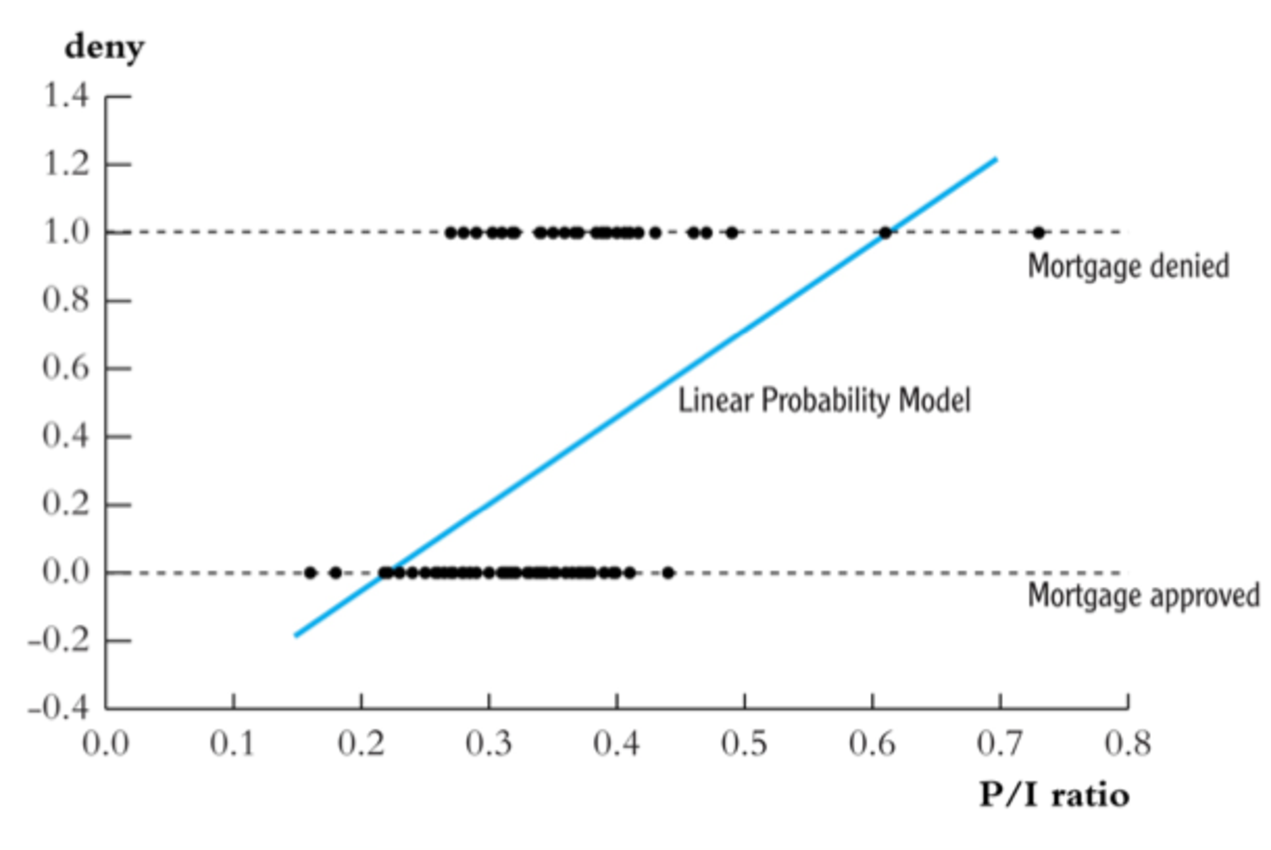
\includegraphics[width=5in]{resources/lpm.pdf}\\
\end{center}
\end{frame}


\begin{frame}
\frametitle{Binary Choice: Overview}
Many problems we are interested in look at discrete rather than continuous outcomes.
\begin{itemize}
\item We are familiar with limitations of the linear probability model (LPM)
\begin{itemize}
\item Predictions outside of $[0,1]$
\item Estimates of marginal effects need not be consistent.
\end{itemize}
\item What about the case where $Y$ is binary and a regressor $X$ is endogenous?
\begin{itemize}
\item The usual 2SLS estimator is \alert{NOT consistent}.
\item Or we can ignore the fact that $Y$ is binary...
\item Neither seems like a good option
\end{itemize}
\item Suppose we have panel data on repeated binary choices
\begin{itemize}
\item Adding FE to the probit model produces biased estimates.
\end{itemize}
\end{itemize}
\end{frame}
\begin{frame}
\frametitle{Problem \#1: Endogeneity}
Four possible solutions (maybe there are more?)
\begin{enumerate}
\item Close eyes, run the LPM with instruments (Suggested by MHE).
\item Specify the distribution of errors in first and second stage and do MLE (\texttt{biprobit} in STATA).
\item Control Function Estimation
\item `Special Regressor' Methods
\end{enumerate}
\end{frame}

\begin{frame}{Linear Probability Model}
First thing we might try is OLS
\begin{eqnarray*}
Y_i  = \beta_0 + \beta_1 X_i + \varepsilon_i
\end{eqnarray*}
\begin{itemize}
\item What does $\beta_1$ mean when $Y$ is binary? Is $\beta_1  = \frac{\Delta Y}{\Delta X}$?
\item What does the line $\beta_0 + \beta_1 X$ when $Y$ is binary?
\item What does the predicted value $\hat{Y}$ mean when $Y$ is binary? Does $\hat{Y} = 0.26$ mean that someone gets approved or denied for a loan?
\end{itemize}
\end{frame}

\begin{frame}{Linear Probability Model}
OLS is called the \alert{linear probability model} 
\begin{eqnarray*}
Y_i  = \beta_0 + \beta_1 X_i + \varepsilon_i 
\end{eqnarray*}
because:
\begin{eqnarray*}
E[Y | X] &=& 1 \times Pr(Y=1 | X) + 0 \times Pr(Y=0  | X) \\
Pr(Y=1 | X) &=& \beta_0 + \beta_1 X_i + \varepsilon_i
\end{eqnarray*}
The predicted value is a \alert{probability} and 
\begin{eqnarray*}
\beta_1 = \frac{Pr(Y=1 | X =x+\Delta x) - Pr(Y=1 | X=x)}{\Delta x}
\end{eqnarray*}
So $\beta_1$ represents the average change in probability that $Y=1$ for a unit change in $X$.
\end{frame}



\begin{frame}
\frametitle{Problem \#1: Endogeneity}
Setup:
\begin{itemize}
\item Binary variable $D$: the outcome of interest
\item $X$ is a vector of observed regressors with coefficient $\beta$ 
\begin{itemize}
\item (Can think about $X^e$: endogenous and $X^0$: exogenous).
\item In an treatment model we might have that $T$ is a binary treatment indicator within $X$
\end{itemize}
\item $\epsilon$ is unobserved error. Specifying $f(e)$ can give logit/probit.
\item Threshold Crossing / Latent Variable Model:
\begin{eqnarray*}
D = \mathbf{1}(X \beta + \epsilon \geq 0)
\end{eqnarray*}
\item Goal is not usually $\hat{\beta}$ or it's CI, but rather $P(D=1 | X)$ or $\frac{\partial P[D=1 | x] }{\partial X}$ (marginal effects).
\end{itemize}
\end{frame}


\begin{frame}
\frametitle{Linear Probability Model}
Consider the LPM with a single continuous regressor
\begin{itemize}
\item LPM prediction departs greatly from CDF long before $[0,1]$ limits.
\item We get probabilities that are too extreme even for $X\hat{\beta}$ ``in bounds''.
\item Some (MHE) argue that though $\hat{Y}$ is flawed, constant marginal effects are still OK.
\end{itemize}
\begin{center}
\includegraphics[width=2in]{resources/lpm-probit.jpg}
\end{center}
\end{frame}

\begin{frame}{Some well known textbooks}
(Baby) Wooldrige:
\begin{quote}
``Even with these problems, the linear probability model is useful and often applied in economics. It usually works well for values of the independent variables that are near the averages in the sample.'' (2009, p. 249)
\end{quote}
\begin{itemize}
\item Mentions heteroskedasticity of error (which is binomial given $X$) but does not address the violation of the first LSA.
\end{itemize}
\end{frame}

\begin{frame}{Some well known textbooks}
Angrist and Pischke (MHE) 
\begin{itemize}
\item several examples where marginal effects of probit and LPM are ``indistinguishable''.
\end{itemize}

\begin{quote}
...while a nonlinear model may fit the CEF (conditional expectation function) for LDVs (limited dependent variable models) more closely than a linear model, when it comes to marginal effects, this probably matters little. This optimistic conclusion is not a theorem, but as in the empirical example here, it seems to be fairly robustly true.(2009, p. 107)
\end{quote}
and continue...
\begin{quote}
...extra complexity comes into the inference step as well, since we need standard errors for marginal effects. (ibid.)
\end{quote}
\end{frame}

\begin{frame}
\frametitle{Linear Probability Model}
How does the LPM work?
\begin{eqnarray*}
D = X \beta + \varepsilon
\end{eqnarray*}
\begin{itemize}
\item Estimated $\hat{\beta}$ are the MFX.
\item With exogenous $X$ we have $E[D | X] = Pr[D=1 | X] = X \beta$.
\item If some elements of $X$ (including treatment indicators) are endogenous or mismeasured they will be correlated with $E$.
\item In that case we can do IV via 2SLS or IV-GMM given some instruments $Z$.
\item We need the usual $E[\varepsilon  | X]= 0 $ or $E[\varepsilon | Z] = 0$. \pause
\item An obvious flaw: Given any $\varepsilon | X  $ must equal either $1- X \beta$ or $-X \beta$ which are functions of $X$
\item \alert{Only the trivial binary $X$ with no other regressors satisfies this!}
\end{itemize}
\end{frame}

\begin{frame}
\frametitle{Alarming Example: Lewbel Dong and Yang (2012)}
\begin{itemize}
\item LPM is not just about taste and convenience.
\item Three treated observations, three untreated % \texttt{Treated=1}
\item Assume that $f(\varepsilon) \sim N(0,\sigma^2)$
\begin{eqnarray*}
D = I ( 1 + Treated + R + \varepsilon \geq 0 ) 
\end{eqnarray*}
\item Each individual treatment effect given by:
\begin{eqnarray*}
 I ( 2 + R + \varepsilon \geq 0 ) -  I ( 1 + R + \varepsilon \geq 0 )  =  I ( 0 \leq 1 + R + \varepsilon \leq 1 ) 
\end{eqnarray*}
\item All treatment effects are positive for all $(R,\varepsilon)$.
\item Construct a sample where true effect $=1$ for 5th individual, 0 otherwise. $ATE= \frac{1}{6}$.
\end{itemize}
\end{frame}

\begin{frame}[fragile]
\frametitle{Alarming Example: Lewbel Dong and Yang (2012)}
\tiny
\begin{semiverbatim}
. list
     |     R   Treated   D |
  1. |  -1.8         0   0 | 
  2. |   -.9         0   1 |
  3. |  -.92         0   1 |
  4. |  -2.1         1   0 |
  5. | -1.92         1   1 |
  6. |    10         1   1 |

. reg D Treated R, robust

Linear regression                               Number of obs     =          6
                                                F(2, 3)           =       1.02
                                                Prob > F          =     0.4604
                                                R-squared         =     0.1704
                                                Root MSE          =     .60723

------------------------------------------------------------------------------
             |               Robust
           D |      Coef.   Std. Err.      t    P>|t|     [95% Conf. Interval]
-------------+----------------------------------------------------------------
     Treated |  -.1550841   .5844637    -0.27   0.808    -2.015108     1.70494
           R |   .0484638   .0419179     1.16   0.331    -.0849376    .1818651
       _cons |   .7251463   .3676811     1.97   0.143    -.4449791    1.895272
------------------------------------------------------------------------------
. nlcom _b[Treated]/_b[R]
       _nl_1:  _b[Treated]/_b[R]
------------------------------------------------------------------------------
           D |      Coef.   Std. Err.      z    P>|z|     [95% Conf. Interval]
-------------+----------------------------------------------------------------
       _nl_1 |       -3.2   10.23042    -0.31   0.754    -23.25125    16.85125
------------------------------------------------------------------------------
\end{semiverbatim}
\end{frame}

\begin{frame}[fragile]
\frametitle{Alarming Example: Lewbel Dong and Yang (2012)}
\begin{itemize}
\item That went well, except that:
\begin{itemize}
\item we got the wrong sign of $\beta_T$
\item $\beta_1/\beta_2$ was the wrong sign and three times too big.
\end{itemize}
\item this is not because of small sample size or $\beta_1 \approx 0$.
\item As $n \rightarrow \infty$ we can get an arbitrarily precise wrong answer.
\item We don't even get the sign right!
\item This is still in OLS (not much hope for 2SLS).
\end{itemize}
\tiny
\begin{semiverbatim}
. expand 30
(...)
. reg D Treated R, robust

Linear regression                               Number of obs     =        180
                                                F(2, 177)         =      59.93
                                                Prob > F          =     0.0000
                                                R-squared         =     0.1704
                                                Root MSE          =       .433

------------------------------------------------------------------------------
             |               Robust
           D |      Coef.   Std. Err.      t    P>|t|     [95% Conf. Interval]
-------------+----------------------------------------------------------------
     Treated |  -.1550841   .0760907    -2.04   0.043    -.3052458   -.0049224
           R |   .0484638   .0054572     8.88   0.000     .0376941    .0592334
       _cons |   .7251463    .047868    15.15   0.000     .6306808    .8196117
\end{semiverbatim}
\end{frame}

\begin{frame}
\frametitle{Solution \#0 : LPM}

\begin{block}{Advantages}
\begin{itemize}
\item Just like 2SLS.
\item Computationally easy (no numerical searches)
\item Missing $Z$ is about efficiency not consistency.
\item $X^e$ can be discrete or continuous (same estimator)
\item allows general heteroskedasticity (random coefficients)
\end{itemize}
\end{block}

\begin{block}{Disadvantages}
\begin{itemize}
\item $\hat{F}_D$ is linear not S-shaped, approximation valid for small range of $X$.
\item $\hat{F}_D$ can be outside $[0,1]$.
\item no element of $X$ can have $\infty$ support (e.g. no normally distributed regressors).
\item $\varepsilon$ not independent of any regressors  (even the exogenous ones). How do we also get $E[X^0 \varepsilon] =0$ ?
\item Does not nest probit, logit, etc.. Can't compare efficiency
\end{itemize}
\end{block}

\end{frame}



\begin{frame}
\frametitle{Solution \#1 : MLE}
\begin{eqnarray*}
D = I ( X' \beta + \varepsilon \geq 0 ) \quad \mbox{and} \quad X^e = G(Z,\theta,e)
\end{eqnarray*}
\begin{itemize}
\item Fully specified $G$ (could be vector). Could be linear if $X^e$ continuous or probit if $X^e$ binary.
\item Need to fully specify distribution of $(\varepsilon,e, | Z)$, parametrized.
\item Implementation (see book), \texttt{biprobit} for joint normal in Stata.
\end{itemize}
\end{frame}


\begin{frame}
\frametitle{Solution \#1 : MLE}

\begin{block}{Advantages}
\begin{itemize}
\item Nests logit, probit, etc. as special cases.
\item Can have any kind of $X^e$
\item Allows heteroskedasticity, random coefficients
\item Asymptotically efficient (if correctly specified)
\end{itemize}
\end{block}

\begin{block}{Disadvantages}
\begin{itemize}
\item Need to parametrize everything $G$, $F_{\varepsilon,e|Z}$.
\item Numerical optimization issues
\item Many nusiance parameters, sometimes poorly identified, especially with discrete $X^e$, correlation between latent $(\varepsilon,e)$.
\item Need to know all required instruments $Z$. Omitting just one $Z$ causes inconsistency in $G$. (Not sure if something is exogenous, too bad!).
\end{itemize}
\end{block}
\end{frame}

\begin{frame}
\frametitle{Solution \#2 : Control Functions}
\begin{eqnarray*}
D &=& I ( X' \beta + \varepsilon \geq 0 ) \quad \mbox{and} \\
 X^e &=& G(Z) +e  \quad \mbox{or}  \quad  X^e = G(Z,e) \quad \mbox{ identified and invertible in $e$}\\
  \varepsilon  &=&\lambda' e + U \quad \mbox{or}  \quad  \varepsilon = H(U,e) \quad \mbox{ with conditions and } U \bot Z,e.
\end{eqnarray*}
Simple Case:
\begin{itemize}
\item Estimate a vector of functions $G$ in the $X^e$ models, get estimated errors $\hat{e}$.
\item Estimate the $D$ model including $\hat{e}$ as additional regressors in addition to $X$.
\item This ``cleans'' the errors in $U$.
\end{itemize}
\end{frame}



\begin{frame}
\frametitle{Solution \#2 : Control Functions (Stata Version)}
\begin{itemize}
\item \texttt{ivprobit} assumes that $G(Z,e)$ is linear, and $(e,\varepsilon)$ jointly normal, independent of $Z$.
\item not exactly the semi-parametric flexibility we were looking for...
\item It is actually Control Function not IV
\end{itemize}
\begin{eqnarray*}
D &=& I ( X^e  \beta_e + X^0 \beta_0+ \varepsilon \geq 0 ) \\
 X^e &=& \gamma Z + e  
\end{eqnarray*}
Run first-stage OLS and get residuals $\hat{e}$. Then plug into
\begin{eqnarray*}
D &=& I ( X^e  \beta_e + X^0 \beta_0+ + \lambda \hat{e} + U  \geq 0 )
\end{eqnarray*}
and do a conventional probit estimator.
\begin{itemize}
\item If you forget a $Z_2$ the resulting model isn't even probit!
\item God help you if $X^e$ isnt continuous.
\end{itemize}

\end{frame}



\begin{frame}
\frametitle{Solution \#2 : Control Functions}
\begin{eqnarray*}
D &=& I ( X' \beta + \varepsilon \geq 0 ) , \quad X^e = G(Z,e) ,  \varepsilon = H(U,e),  \quad U \bot X,e.
\end{eqnarray*}
Much stronger requirements that 2SLS
\begin{itemize}
\item Must be able to solve for errors $e$ in $X^e$ equations (not just orthogonality)
\item Endogeneity must be caused only by $\varepsilon$ relation to $e$ so after conditioning on $e$ must be that $f(\varepsilon | e, X^{e}) = f( \varepsilon | e)$.
\item I need a consistent estimator for $e$ which means nothing is omitted.
\end{itemize}
Not Quite MLE
\begin{itemize}
\item First stage can be semi/non-parametric .
\item Don't need to fully specify joint distribution of $(\varepsilon,e)$ (Stata does though!).
\end{itemize}


\end{frame}


\begin{frame}
\frametitle{Solution \#2 : Control Functions}
\begin{block}{Advantages}
\begin{itemize}
\item Nests logit, probit, etc. as special cases
\item Requires less parametric information than MLE
\item Some versions are computationally easy without numerical optimization (Bootstrap!)
\item Less efficient than MLE due to less restrictions,but can be semiparametrically efficient given information.
\end{itemize}
\end{block}
\end{frame}

\begin{frame}
\frametitle{Solution \#2 : Control Functions (Disadvantages: Not well known)}
\begin{itemize}
\item Only allows limited heteroskedasticity
\item Need to correctly specify vector $G(Z,e)$ including all $Z$. Omitting a $Z$ or misspecified $G$ causes inconsistency because we need to have joint conditions on $(\varepsilon , e)$.
\item Generally inconsistent for $X^e$ that is discrete, censored, limited, or not continuous.
\item If you cannot solve for a latent $e$ in $G(Z,e)$ then you can't get $\hat{e}$ for the censored observations (e.g.: $X^e = \max(0, Z'\gamma + e)$.
\item An observable $e$ is $e = X^e - E[X^e | Z]$ but for discontinuous $X^e$ that $e$ violates assumptions (except in very strange cases)
\begin{itemize}
\item Ex: $\varepsilon =  [ X^e - E[X^e | Z]] \lambda + U$ satisfies CF, but if $X^e$ is discrete then $e$ has some strange distribution that depends on regressors. 
\item Hard to generate a model of behavior that justifies this!
\end{itemize}
\end{itemize}
\end{frame}



\begin{frame}
\frametitle{Solution \#2 : Control Functions Generalized Residuals}
What if $X^e$ isn't continuous? Technically possible...
\begin{itemize}
\item Given the probit estimate in first stage we could construct a generalized residual (see Imbens and Wooldridge notes) 
\item $e^g \propto E[\varepsilon | Z, e]$. An estimate $\hat{e}^g$ of $e^g$ can be included as a regressor in the model to fix the endogeneity problem, just as $\hat{e}$ would have been used if the endogenous regressor were continuous.
\end{itemize}
Why would you ever want to do this..
\begin{itemize}
\item In the linear model we should just do IV with far fewer restrictions
\item In the nonlinear model, $\hat{e}^g$ requires almost as many assumptions as MLE which is efficient!
\end{itemize}
\end{frame}

\begin{frame}
\frametitle{Solution \#3 : Special Regressor}
This approach draws on these two papers:
\begin{itemize}
\item Lewbel (JoE 2002)
\item Dong and Lewbel (Econometric Reviews 2015)
\end{itemize}
\begin{eqnarray*}
D &=& I ( X' \beta + V + \varepsilon \geq 0 )
\end{eqnarray*}
Special Regressor $V$ has three properties
\begin{itemize}
\item Exogenous $E[\varepsilon | V ] =0$
\item Additively separable in the model
\item Continuous distribution and large support (such as Normal)
\item Helpful to have thick-tails (kurtosis). Why? We want to trace $Pr(D | V)$ from $[0,1]$.
\end{itemize}
\end{frame}

\begin{frame}{Learn about SR}
\small
Binary, ordered, and multinomial choice, censored regression, selection, and treatment models (Lewbel 1998, 2000, 2007a), truncated regression models (Khan and Lewbel 2007), binary panel models with FE (Honore and Lewbel 2002), dynamic choice models (Heckman and Navarro 2007, Abbring and Heckman 2007), contingent valuation models (Lewbel, Linton, and McFadden 2008), market equilibrium models of multinomial choice (Berry and Haile 2009a, 2009b), models with (partly) nonseparable errors (Lewbel 2007b, Matzkin 2007, Briesch, Chintagunta, and Matzkin 2009).\\
Other empirical applications: Anton, Fernandez Sainz, and Rodriguez-Poo (2002), Cogneau and Maurin (2002), Goux and Maurin (2005), Stewart (2005), Lewbel and Schennach (2007), and Tiwari, Mohnen, Palm, and van der Loeff (2007).\\
Precursors: Matzkin (1992, 1994) and Lewbel (1997).\\
Recent theory: Magnac and Maurin (2007, 2008), Jacho-Ch�vez (2009), Khan and Tamer (2010), and Khan and Nekipelov (2010a, 2010b).
\end{frame}


\begin{frame}
\frametitle{Solution \#3 : Special Regressor}
Requirements:
\begin{eqnarray*}
D &=& I ( X' \beta + V + \varepsilon \geq 0 )
\end{eqnarray*}
\begin{itemize}
\item Exogenous $E[\varepsilon | V ] =0$ (Strict Exogeneity) \alert{This is the key!} 
\item Additively separable in the model
\item Continuous distribution and large support (such as Normal)
\item NOT interacted with other regressors.
\item enters LINEARLY, e.g. $V$ must be continuously distributed after conditioning on other regressors
\item Can normalize its coefficient to $1$
\item 2SLS Assumptions: $E[ \varepsilon | Z] = 0$ and $E[Z'X]$ is full rank.
\end{itemize}
\end{frame}

\begin{frame}
\frametitle{Solution \#3 : Special Regressor: How it works}
\begin{enumerate}
\item Demean or center $V$ at zero. 
\item Assume that $f_v ( V | Z,X^e) = f_v(V | Z)$ and let $\hat{f}_v ( V | Z) $ be a nonparametric kernel estimator of $f_v(V | Z)$. Or just use a kernel of the whole thing $\hat{f}_v ( V | Z,X^e)$
\item For each observation $i$, Construct $\hat{T}_i = I [D_i -  I(V_i \geq 0)]/ \hat{f_v} (V_i | Z_i)$
\item Linear 2SLS regression of $\hat{T}$ on $X$ using instruments $Z$ to get the estimated coefficients $\hat{\beta}$.
\end{enumerate}
Here $\hat{f}_v(V|Z)$ is high dimensional. So will consider some simpler parametric or semi-parametric version of $f_v$.\\
By properly adjusting $T_i$ we guarantee to stay in $[0,1]$.
\end{frame}




\begin{frame}
\frametitle{Solution \#3 : Special Regressor Advantages}
\begin{itemize}
\item Unlike LPM it stays ``in bounds'' and is consistent with threshold crossing models.
\item Unlike MLE and CF, does not require correctly specified first stage model: any valid set of instruments may be used, with only efficiency at stake.
\item Unlike MLE, the SR method has a linear form, not requiring iterative search
\item Unlike CF, the SR method can be used when endogenous regressors $X^e$ are discrete or limited; unlike ML there is a single estimation method, regardless of the characteristics of $X^e$
\item Unlike MLE, the SR method permits unknown heteroskedasticity in the model errors.
\end{itemize}
\end{frame}

\begin{frame}
\frametitle{Solution \#3 : Special Regressor Disadvantages}
\begin{eqnarray*}
D &=& I ( X' \beta + V + \varepsilon \geq 0 )
\end{eqnarray*}
\begin{itemize}
\item Because assumptions are weaker we give up a lot of potential efficiency (larger SEs).
\item Of course this presumes the assumptions were valid and alternatives were consistent.
\item SR Methods are generally valid under more general conditions.
\end{itemize}
\end{frame}

\begin{frame}
\frametitle{ The average index function (AIF)/ Propensity Score}
In the original problem
\begin{eqnarray*}
D &=& I ( X' \beta + \varepsilon \geq 0 )
\end{eqnarray*}
\begin{itemize}
\item $V$ is part of $X$ with coefficient $=1$
\item When $\varepsilon \bot x$ write the propensity score: $E[D | X] = E[D | X \beta] = F_{-\varepsilon} (X \beta)  = Pr(- \varepsilon \leq X \beta)$. 
\item Under independence $X \bot \varepsilon$ these are the same, under endogeneity or even heteroskedasticity they are not.
\end{itemize}
\end{frame}

\begin{frame}
\frametitle{ The average index function (AIF)/ Propensity Score}
\begin{itemize}
\item Blundell and Powell (ReStud 2004, this is actually the most important control function paper) use the average structural function (ASF) $= F_{-\varepsilon} (X \beta) $ to summarize choice probabilities. But when $\varepsilon \bot X$ is violated then they have to compute $F_{-\varepsilon | X} (X \beta) $ which is quite difficult (especially semiparametrically).
\item Lewbel, Dong and Tang (CJE 2012) propose using the AIF estimator $E[D | X \beta]$ instead.
\item Like ASF the AIF is based on the estimated index $X \beta$ and is equal to the propensity score if $\varepsilon \bot X$. However, when this is violated (endogeneity, heteroskedasticity) the AIF is easier to estimate, via unidimensional nonparametric regression of $D$ on $X \beta$.
\end{itemize}
\end{frame}

\begin{frame}
\frametitle{ What is the difference}
\begin{description}
\item[Propensity Score: ]  Conditions on ALL covariates using $F_{-\varepsilon | X}$.
\item[ASF: ]  Conditions on no covariates using $F_{-\varepsilon }$.
\item[AIF: ]  Conditions on index only  using $F_{-\varepsilon | X \beta}$.
\end{description} 

\begin{itemize}
\item Unlike ASF, AIF is always identified and easy to estimate.
\item Unlike Propensity score AIF uses $\beta$ and isn't high dimensional
\item ASF, AIF and propensity score all coincide under exogeneity.
\end{itemize}
\end{frame}

\begin{frame}
\frametitle{ Marginal Effects}
\begin{itemize}
\item With exogenous $X$: MFX are $m(X) = p'(X) =  \frac{\partial E[D | X \beta]}{\partial X}$.
\item Let $f_{-\varepsilon}$ be marginal pdf of $-\varepsilon$. If $D=I(X' \beta + \varepsilon \geq 0)$ with $\varepsilon \bot X$ then:
\end{itemize}
\begin{eqnarray*}
m (X \beta) \beta= \frac{\partial E[D | X]}{\partial X}  = \frac{\partial E[D | X \beta]}{\partial X' \beta}  \beta  = f_{-\varepsilon}(X' \beta) \beta
\end{eqnarray*}

With endogenous $X$:
\begin{itemize}
\item Propensity Score marginal effects are $m(X) = p'(X) =  \frac{\partial E[D | X]}{\partial X}$.
\item ASF marginal effects are $m(X) =\frac{\partial ASF(X'\beta)}{\partial X'\beta} \beta = f_{-\varepsilon}(X' \beta) \beta.$
\item AIF marginal effects are $m(X) =\frac{\partial ASF(X'\beta)}{\partial X'\beta} \beta = \frac{\partial E[D | X' \beta ]}{\partial X' \beta} \beta$
\end{itemize}
Given $\hat{\beta}$ ASF and AIF mfx require just one dimensional index derivative.
\end{frame}

\begin{frame}
\frametitle{Binary Choice with Endogenous Regressors}
\begin{itemize}
\item Linear probability models, Maximum Likelihood, and Control functions (including \texttt{ivprobit} have more drawbacks and limitations than are usually recognized.
\item Special Regressor estimators are a viable alternative (or at least they have completely different drawbacks and may be more generally applicable than has been recognized).
\item In practice, best might be to try all estimators and check robustness of results. Can use marginal effects to normalize them the same when comparing.
\item Average Index Functions can be used to construct estimated probabilities and comparable marginal effects across estimators, often simpler to calculate than Average Structural Functions.
\item Implementation of special regressor in Stata is done in \texttt{sspecialreg}.
\end{itemize}
\end{frame}

\begin{frame}
\frametitle{Empirical Example: Dong and Lewbel (2015)}
\begin{itemize}
\item Binary dependent variable: does $i$ migrate from one state to another. 
\item Special Regressor $V_i$: age. Human capital theory suggests it should appear linearly (or at least monotonic) in a threshold crossing model 
\item Migration is drive by maximizing expected lifetime income and potential gain from a permanent change in income declines linearly in age.
\item $V_i$ is defined as negative of age, demeaned so that coefficient is positive with mean zero.
\item Other endogenous regressors: family income pre migration, home ownership.
\end{itemize}
\end{frame}

\begin{frame}
\frametitle{Empirical Example: Dong and Lewbel (2015)}
As a reminder, normally we would be in trouble here:
\begin{itemize}
\item MLE would be very complicated with multiple endogenous variables
\item Control functions \texttt{ivprobit} won't work with 0/1 homeowner variable.
\end{itemize}
\end{frame}

\begin{frame}
\frametitle{Empirical Example: Dong and Lewbel (2015)}
1990 PSID
\begin{itemize}
\item male head of household (23-59 years), completed education and not-retired (key!)
\item $D=1$ indicates migration during 1991-1993.
\item 4689 Individuals, 807 migrants.
\item Exogenous regressors: years of education, \# of children, white, disabled, married.
\item Instruments: level of govt benefits in 1989-1990, state median residential tax rate.
\end{itemize}
\end{frame}

\begin{frame}
\frametitle{Empirical Example: Dong and Lewbel (2015)}
Specifications
\begin{itemize}
\item Special Regressors: kernel density vs. sorted data density.
\item Special Regressor: homoskedastic vs. heteroskedastic errors.
\item LPM vs 2SLS
\item Probit (assuming exogeneity)
\item Control Function (\texttt{ivprobit}) misspecified for \texttt{homeowner} endogenous binary variable.
\end{itemize}
\end{frame}


\begin{frame}
\frametitle{Empirical Example}
\begin{center}
\includegraphics[width=4in]{resources/specialregtable.png}
\end{center}
\end{frame}

\begin{frame}
\frametitle{Empirical Example: Dong and Lewbel (2015)}

\begin{itemize}
\item SEs of MFX are computed from 100 bootstrap replications
\item MFX of special regressor (age) is estimated as positive and significant but LPM and ivprobit estimate negative effects!
\item household income and home ownership status do not seem to play significant roles in migration decision.
\item Kernel density estimator seems to give most significant results.
\end{itemize}
\end{frame}


\end{document}
